\documentclass{beamer}
\usepackage{amsmath}
\usepackage{amssymb}
\usepackage{mathrsfs}
%\usepackage{biblatext}
\usepackage{graphicx} %for inserting images
\graphicspath{ {./images/} }  % folder where images file is
\usepackage[autostyle]{csquotes}
\usetheme{Warsaw}
%\usetheme{CambridgeUS}
%\usetheme{Madrid}
%\usetheme{Pittsburgh}
\title{A hybrid cryptographic system for file security}
\subtitle{}

\author{\textit{Presented by:} Group-H}


\titlegraphic{
	
\includegraphics[width=0.3\textwidth, height=0.3\textwidth]{TIT}
}
	
\institute[TIT]{
Dept. Of Computer Science and Engineering\\
Tripura Institute of Technology, Narsingarh\\
\medskip
}
\date{}

\begin{document}

\begin{frame}
\titlepage
\end{frame}

\begin{frame}[t]
	\frametitle{Group-H}
	\large \textbf{Team Members: }\\
	\begin{itemize}
		\item Hamjak Debbarma [27/CS/L/23/47]
		\item Joydeep Saha  [27/CS/L/23/56]
		\item Raju Debnath  [27/CS/23/12]
	\end{itemize}
\vspace{0.5in}
 \large \textbf{Supervised By: }  Prof. Pankaj Debbarma\\
\end{frame}


\begin{frame}
\frametitle{Outline}
\begin{itemize}
\item Problem Statement
\item Solution
\item Hybrid Cryptography 
\item RSA Algorithm
\item KASUMI Cipher
\item Proposed System Design 
\item Advantages of Proposed System 
\item Implementation
\item Further Work
\item References
\end{itemize}
\end{frame}

\begin{frame}
	\frametitle{Problem Statement}
	\begin{itemize}
		\item In this information and digital age, we generate a lots of data
		\item Many personal documents and important business files are shared across all over the internet
		\item All these are vulnerable to attack and information breaches.
	\end{itemize}
\end{frame}

\begin{frame}
	\frametitle{Solutions}
	The solution is to build secure encryption system using the secure cryptographic algorithms that could withstand various attacks.
\end{frame}

\begin{frame}
\frametitle{Hybrid Cryptography}
 The ISO/LEC JTCI/SC27 standardization committee suggests that hybrid cryptography can be defined as the branch of asymmetric cryptography that makes use of convenient symmetric techniques to remove some of the problems inherent in normal asymmetric cryptosystem.
\end{frame}

\begin{frame}
\frametitle{Hybrid Cryptography}
\textbf{Hybrid Cryptography} is the combination of both the symmetric key cryptography and Asymmetric or Public key cryptography.
\end{frame}

\begin{frame}
	\frametitle{Hybrid Cryptography}
	Our Goal: to build a hybrid cryptosystem using the following algorithms:
	\vspace{0.2in}
	\begin{itemize}
		\item RSA Algorithm (Asymmetric)
		\item KASUMI Cipher (Symmetric)
	\end{itemize}
\end{frame}

\begin{frame}[t]
	\frametitle{RSA Algorithm}
	 \begin{itemize}
	 	\item Public Key Cryptosystem
	 	\item Invented by Rivest, Shamir and Adleman [1977]
	 	\item It is based on the principle that it is easy to multiply large numbers but factoring large number is very difficult.
	 	\item Public key is generated by multiplying two large prime numbers and private key is generated by using a mathematical functions.
	 	\item Key Size : $512$ bits to $4096$ bits
	 	 
	 \end{itemize}
\end{frame}

\begin{frame}[t]
	\frametitle{RSA: Advantages}
	\begin{itemize}
		\item RSA Algorithm involves a lot of complex mathematics which makes it more difficult to crack.
		\item Fast Encryption as compare to other encryption algorithm.
		\item No need of sharing secrets key
		\item Proof of owner's authenticity
		\item Data cannot be modified at transit
	\end{itemize}
\end{frame}
\begin{frame}[t]
	\frametitle{RSA: Disadvantages}
	\begin{itemize}
	\item Key generation is very slow.
	\item Speed of encrypting of text is slow. 
	\item High processing is required at receiver’s end for decryption
	\end{itemize}
\end{frame}

\begin{frame}[t]
	\frametitle{KASUMI Cipher}
	\begin{itemize}
		\item It is a Fiestel Cipher
		\item Based on the MISTY1 Cipher
		\item Mostly used in Universal Mobile Telecomm. System(UMTS), Global System for Mobile Comm. (GSM) and GPRS Mobile Comm.
 		\item Key size: $128$ bits
 		\item Block Size: $64$ bits
 		\item The core of KASUMI is an $8$-round Feistel network.
 		\item In each round the round function uses a round key which consists of eight $16$-bit sub keys derived from the original $128$-bit key using a fixed key schedule.
	\end{itemize}

\end{frame}

\begin{frame}
	\frametitle{KASUMI Cipher}
	\textbf{Working of Round Function:}
	Let's consider key, $K$ is $32$ bit and is divided into eight $4$ bit values $K_1, K_2, \dots K_8$ i.e,
	$$ K = K_1 || K_2 || \dots || K_8$$
	Take $k = 0111$ then subkeys :
	\begin{align*}
		K_1 &= 0111\\
		K_2 &= 1011 \\
		K_3 &= 1101\\
		K_4 &= 1110\\
		K_5 &= 0111\\
		K_6 &= 1011\\
		K_7 &= 1101 \\
		K_8 &= 1110
	\end{align*}
	where, $K_1 = K_5$, $K_2 = K_6$, $K_3 = K_7$ and $K_4 = K_8$ \\

\end{frame}
\begin{frame}[t]
	\frametitle{KASUMI Cipher}
	In KASUMI, round keys are :
	\begin{align*}
		KL_{i,1} &= ROL(K_i,1) \\
		KL_{i,2} &= K^{'}_{i+2} \\
		KO_{i,1} &= ROL(K_{i+1},5) \\
		KO_{i,2} &= ROL(K_{i+5},8) \\
		KO_{i,3} &= ROL(K_{i+6},13) \\
		KI_{i,1} &= K^{'}_{i+4} \\
		KI_{i,2} &= K^{'}_{i+3} \\
	    KI_{i,3} &= K^{'}_{i+7} 
	\end{align*}
\end{frame}

\begin{frame}
	\frametitle{KASUMI Cipher}
	%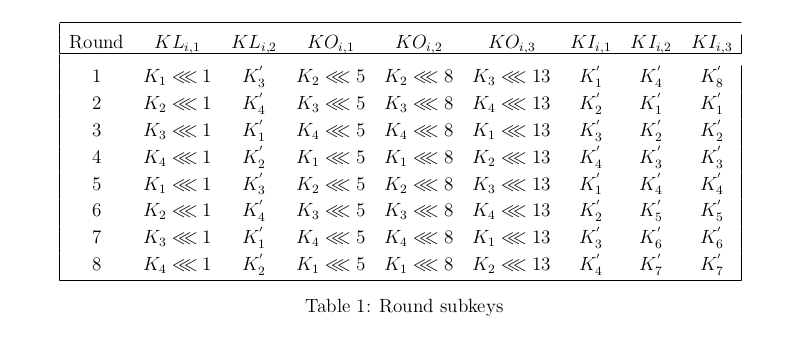
\includegraphics[height=0.5\textwidth>,width=1\textwidth>]{rk}
	\begin{figure}[h]
		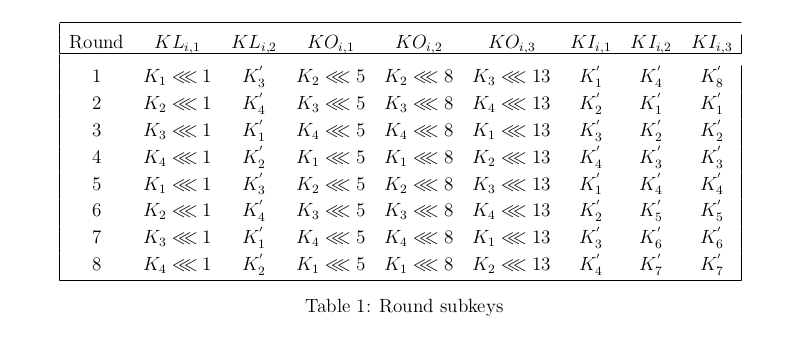
\includegraphics[width=12cm]{rk}
	\end{figure}
\end{frame}

\begin{frame}[t]
	\frametitle{KASUMI: Advantages and Disadvantages}
	\textbf{Advantages: }
	\begin{itemize}
		\item High diffusion and strong tamper resistance without detection
		\item More secure as compare to MISTY1
	\end{itemize}
\textbf{Disadvantages: }
\begin{itemize}
	\item An impossible differential attack[1] on six rounds of KASUMI was presented by Kühn [2001]
	\item A related-key rectangle (boomerang) attack[2] on KASUMI that can break all 8 rounds faster than exhaustive search was published by Eli Biham, Orr Dunkelman and Nathan Keller[2005]
\end{itemize}
\end{frame}

\begin{frame}
	\frametitle{Proposed System Design: Encryption}
	\begin{figure}[h]
		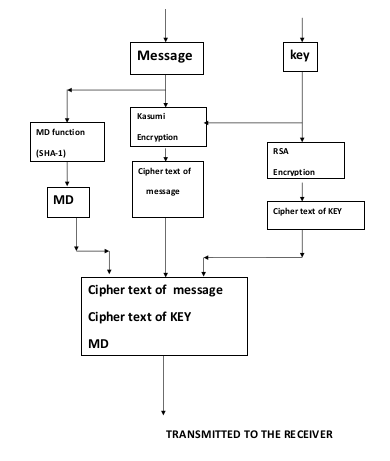
\includegraphics[width=7cm]{en}
	\end{figure}
\end{frame}
	
\begin{frame}
	\frametitle{Proposed System Design: Decryption}
	\begin{figure}[h]
		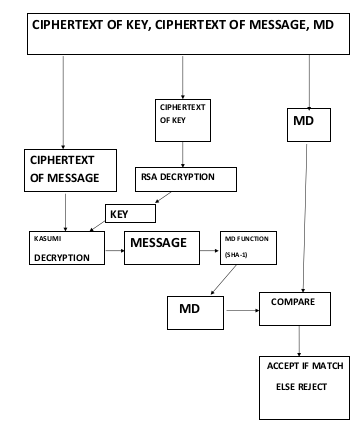
\includegraphics[width=7cm]{de}
	\end{figure}
	
\end{frame}

\begin{frame}[t]
	\frametitle{Advantages of proposed system}
	\begin{itemize}
		\item File is secure as the file is being encrypted not by just using one but two highly algorithms RSA and KASUMI. 
		\item The key used for encryption is also safe as it is encrypted by RSA
		\item Confidentiality and integrity of a file is being maintain securely as Hasing algorithm is used for generating checksum 
	\end{itemize}
\end{frame}

\begin{frame}[t]
	\frametitle{Implementation}
	For the proof of concept and for the demonstration we will be considering:
	\begin{itemize}
		\item Key Size: $32$-bit instead of $128$-bit
		\item Block Size: $16$-bit instead of $64$-bit
	\end{itemize}
\vspace{0.5in}
\textbf{Technologies used: } PHP and SQL
\end{frame}

\begin{frame}
	\frametitle{Further Work}
	\begin{itemize}
		\item Improving the Fiestel Round of the KASUMI Cipher for better security
		\item Introduction of another secret key to be used along with MD Function for maximum security.
	\end{itemize}
\end{frame}

\begin{frame}[t]
	\frametitle{References}
	[1] Kühn, Ulrich. Cryptanalysis of Reduced Round MISTY. EUROCRYPT 2001.

	[2] Orr Dunkelman, Nathan Keller, Adi Shamir (2010-01-10). "A Practical-Time Attack on the A5/3 Cryptosystem Used in Third Generation GSM Telephony"
	
	[3] https://en.wikipedia.org/wiki/KASUMI
	
\end{frame}

\begin{frame}
	\frametitle{}
	\center \Large Thank You !
\end{frame}




\end{document}
